% =========================================================================
% CHAPTER 7 — TRANSLATE: DESIGNING EXPERIENTIAL REPRESENTATIONS
% =========================================================================

\chapter{Designing Experiential Representations}
\label{ch:translate}

\noindent
{\rmfamily\itshape
\begin{tabular}[t]{@{}l@{\hspace{0.3cm}}p{12.5cm}@{}}
\textls[50]{\textbf{Addressed:}} &
\textls[50]{Prototype \& Minimum Viable Product · Informational Equivalence · Fidelity \&
Provenance · Design Grammar · Perceptual Mapping · Three Scenes · Sonification}
\end{tabular}
}

\vspace{0.5cm}

Chapter~\ref{ch:data_pipeline} established what there is to represent. This chapter establishes how it is represented, and why those choices are defensible. It documents the three artefacts of the \emph{Living Atlantic} project, the framework governing all three, and the design grammar offered as this thesis's transferable contribution under objective~O2.2.

% -------------------------------------------------------------------------
\section{From Latent Structure to Perceptual Form}
\label{sec:translate-premise}

Chapter~\ref{ch:data_pipeline} established that two linear modes account for $97.86\%$ of the variance in the AMOC vertical profiles, and that a non-linear autoencoder never exceeds the linear decomposition at matched dimensionality (O1.2). The manifold on which the observational record lives is essentially flat, and that fact licenses everything in this chapter: had it been curved, moving through the plane recovered by PCA would pass through states the ocean never occupied. Because it is flat, each month is a point, and animating along the path between months shows real states, not plausible interpolations.\footnote{Under the Baldi--Hornik result, any autoencoder gain over PCA is attributable to curvature alone; the near-zero gap confirms the manifold is flat enough for linear coordinates to stand in for it faithfully \parencite{baldi1989}.} Hypothesis~H2 is therefore not a negative result but the foundation of the representational phase. Without it, the experiential layer would have no epistemic ground.

This is also the sense in which machine learning operates representationally rather than predictively here. The models of Chapter~\ref{ch:data_pipeline} do not forecast; they propose a coordinate system. Following \textcite{iten2020}, extended to interactive exploration by \textcite{camps2019}, the latent representation is treated as an object a human interpreter may examine and inhabit. What this chapter adds is making the latent space perceptible to a viewer who does not know it exists \parencite{sacha2018}.

% -------------------------------------------------------------------------
\section{The Translate Framework}
\label{sec:translate-framework}

Four commitments and one instrument govern all three scenes, stated once here and applied below.

\subsection{Informational Equivalence by Shared Provenance}
\label{subsec:equivalence}

Objective~O2.1 requires that the two conditions --- conventional static (C1) and dynamic-experiential (C2+C3) --- encode the same data, so that any difference observed in evaluation is attributable to form rather than content. \textcite{tversky2002} showed why this is not a formality: the apparent superiority of animated graphics dissolves wherever the animated condition carries information the static one does not\footnote{An earlier version of the project enforced this equivalence through a shared document architecture. Although the study was later redesigned as a between-subjects experiment, the same principle remains: both conditions are generated from the same data bundle and reconstruction pipeline, differing only in the representational choices applied.}

The final study adopts a between-subjects design: each participant is assigned to a single condition and experiences all three scenes within that condition.\footnote{Administered files are \texttt{column-static.html}, \texttt{theengine-static.html} and \texttt{thethreshold-static.html} (C1), and their \texttt{-experiential} counterparts (C2+C3). A third file per scene exposes all conditions behind a toggle for demonstration and is not administered.} This removes the carry-over effects a sequential design would introduce, at the cost of within-person comparison --- an appropriate trade for an exploratory design analysed against a grid fixed before the responses were read \parencite{braunclarke2019}.

Equivalence is therefore guaranteed not by the file structure but by a shared provenance pipeline: both conditions are generated from the same data bundle, reconstruct every profile through the same function, and document every perceivable element in a common provenance ledger.\footnote{\texttt{amoc\_translate\_bundle.json} (schema v1.0.0), \texttt{shared/reconstruct.js} and \texttt{shared/bundle.js} respectively; the ledger is Table~\ref{tab:ledger} in Appendix~\ref{app:code}, which also documents the module architecture and the repository layout.}

\subsection{Fidelity}
\label{subsec:fidelity}

Every value on screen derives from the bundle. Nothing is rescaled for visual effect, and where an aesthetic preference conflicted with the data, the data won.\footnote{The places where this cost something are recorded in Appendix~\ref{app:limits-translate}.} The reconstruction is one equation, shared by every scene and both conditions:

\begin{equation}
\label{eq:reconstruction}
\Psi(z, t) = \overline{\Psi}(z) + \mathrm{pc}_1(t) \cdot B_1(z) + \mathrm{pc}_2(t) \cdot B_2(z)
\end{equation}

where $\overline{\Psi}$ is the record mean, $B_1$ and $B_2$ are the unit basis vectors of the decomposition and $\mathrm{pc}_1$, $\mathrm{pc}_2$ the latent coordinates of month~$t$.\footnote{The bundle also carries EOF loadings --- the same modes scaled into Sverdrups for display of mode shape only. They must never be passed to Equation~\ref{eq:reconstruction}; see Appendix~\ref{app:code}.}

The equivalence claim can be checked against this equation directly: the static condition obtains the empirical mean by evaluating the shared reconstruction with both coefficients set to zero, which returns the stored mean profile exactly. C1 therefore follows the same computational path as the experimental condition while displaying only observed data; the model enters when the curve begins to move.

\subsection{Machine Learning as a Substrate}
\label{subsec:ml-role}

The machine-learning contribution is structural, not generative. The local meridional velocity that drives the particle field is the vertical derivative of the streamfunction:

\begin{equation}
\label{eq:velocity}
v(z, t) \propto \frac{\partial \Psi(z, t)}{\partial z}
\end{equation}

\noindent This is the distinction the streamfunction misconception of \S\ref{sec:res-misconception} turns on: the curve's \emph{height} is cumulative transport, its \emph{slope} is local flow. The model does not draw the profile curve, colour the particles or produce the mean state; the ledger records those as classical.\footnote{The particle field is a derivative of $\Psi$ (Equation~\ref{eq:velocity}) that any analyst could reproduce with a difference operator. The model touches only the coordinate system and the anomaly scores.} What the model supplies is the latent coordinate system along which the profile moves through time, and the identification of the moments that depart from it. The originality claimed is therefore not a new algorithm but an empirical bridge: a learned latent space used as the substrate on which a complex system is made perceptible to a non-expert, with the model's role confined to where the data licenses it and declared element by element (Table~\ref{tab:ledger}).

\subsection{The Design Grammar}
\label{subsec:grammar}

Objective~O2.2 asks for a design grammar mapping machine-learning-derived features onto perceptual dimensions, grounded in the pre-attentive processing and embodied cognition of \S\ref{sec:cognitive-science} and reusable beyond this case. It is stated in Table~\ref{tab:design-grammar} and not restated here.\footnote{Its six principles, in brief: P0, most important information to the most accurate channel \parencite{munzner2014,bertin1983}; P1, ordered magnitude to spatial position \parencite{clevelandmcgill1984}; P2, dynamics to real motion \parencite{sterman2008,cronin2009}; P3, anomaly to density and texture \parencite{bertin1983,ware2021}; P4, uncertainty to animated variability; P5, secondary ordered variable to sound \parencite{hermann2011}.} Each scene records which principles it realises, so that a mapping which fails in evaluation falls on that mapping --- and through it on the principle --- rather than on the artefact as a whole.

\subsection{Symmetry of Framing}
\label{subsec:symmetry}

Within each scene, both conditions import the same framing modules byte-identically: an introduction carrying the scene's driving question, and a context panel giving the data source and a plain-language account of what is measured.\footnote{\texttt{shared/intro-*.js} and \texttt{shared/context-*.js}, one pair per scene. Identity is by import rather than duplication, so the two documents cannot drift apart through an edit to one of them.} The rule governing this material is that both groups may be taught to read the instrument, but neither may be told the reading. Participants learn what $\Psi$ measures and what a sverdrup is, because a viewer who cannot read the units cannot articulate anything; they are never told what the structure means. If the viewer must be told, the translation has failed, and the evaluation would measure the framing text rather than the representation.

Each scene's driving question is what makes this measurable: posed identically to both groups, answered by neither document, and kept visible throughout.\footnote{The three questions are reproduced in Appendix~\ref{app:protocols} in the form administered. Keeping the question visible rather than showing it once is a design decision: without a stated task, a moving representation reads as decoration rather than enquiry.} The symmetry is not a courtesy to the control group; it is what makes the comparison mean anything at all, and it is what expectation~E3.1 tests.

% -------------------------------------------------------------------------
\section{Three Scenes, One Descent}
\label{sec:three-scenes}

The three scenes are made to be experienced in order, and the order is interpretive rather than aesthetic. It follows the vertical image schema that \citet{lakoff1999} identify as a pre-conceptual cognitive resource --- downward as deeper, more hidden, more fundamental. A viewer who meets the latent plane of Scene~II without first inhabiting the column of Scene~I has no referent for the coordinates; one who meets the ensemble spread of Scene~III without having watched the observed trajectory has no baseline against which disagreement registers. Each scene is the condition of the next one's intelligibility --- and, as \S\ref{sec:eval-limitations} records, a confound for any comparison between them.

The scenes are nonetheless separate documents, so that the user survey presents one scene in one condition with no accumulated interaction state.\footnote{Continuity is carried by the written framing preceding each scene and by the order of administration, not by animated transitions between them.} Each is described below by the same six criteria: goal, representational strategy, mapping, conditions, fidelity and expected contribution. Table~\ref{tab:scene-summary} summarises the three at a glance.

\subsection{Scene I: The Column}
\label{subsec:scene-column}

\begin{quote}
\textbf{Driving Question.} \emph{Does the water move all in the same way? If not --- how, and in which directions, does it move?}
\end{quote}

\begin{figure}[htbp]
  \centering

  \begin{subfigure}{0.48\textwidth}
    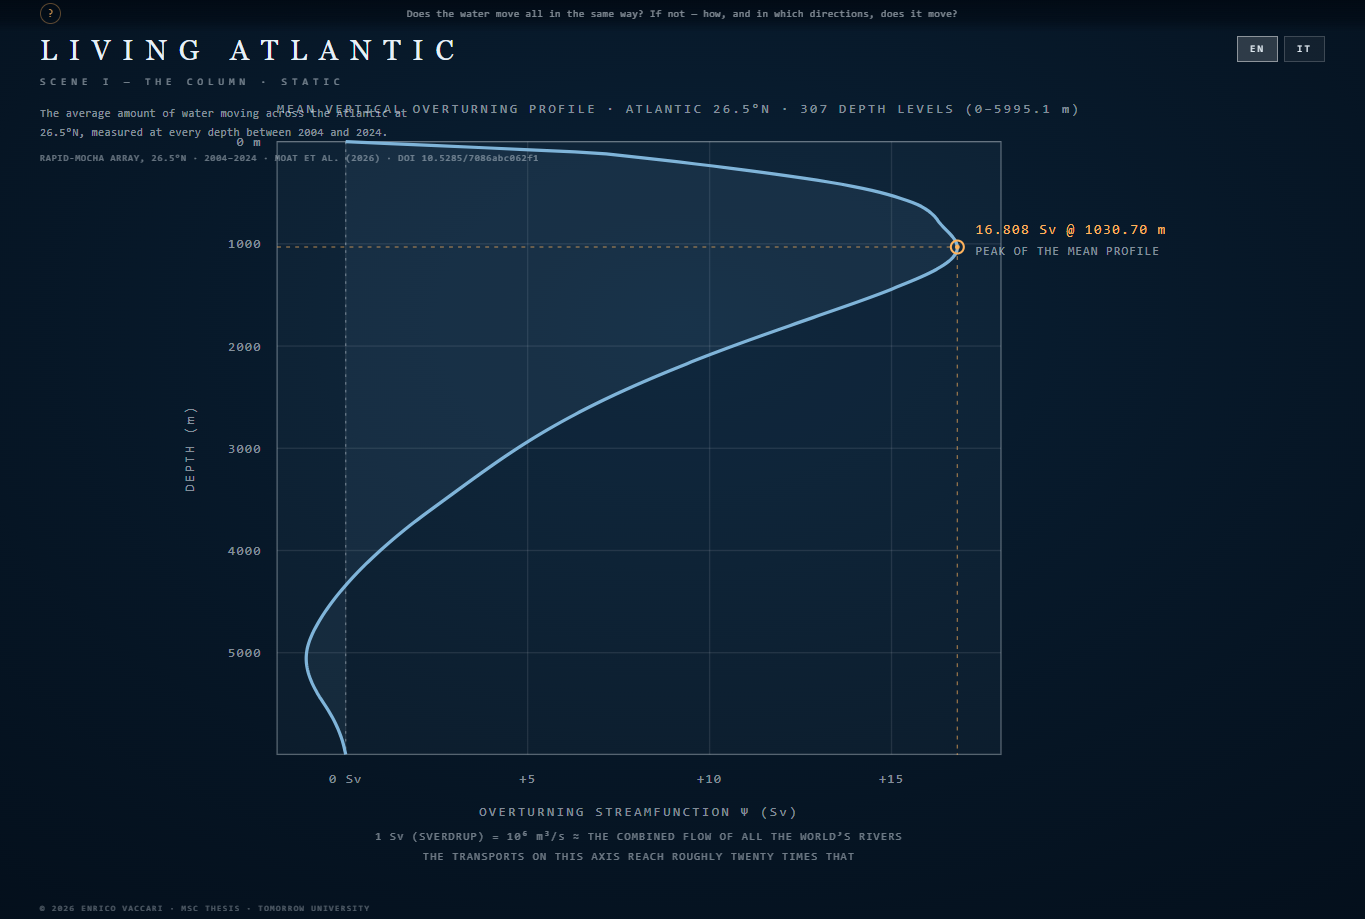
\includegraphics[width=\textwidth]{figures/viz1/viz1_thecolumn-static.png}
    \caption{Control (C1): the canonical static profile.}
    \label{fig:thecolumn-static}
  \end{subfigure}
  \hfill
  \begin{subfigure}{0.48\textwidth}
    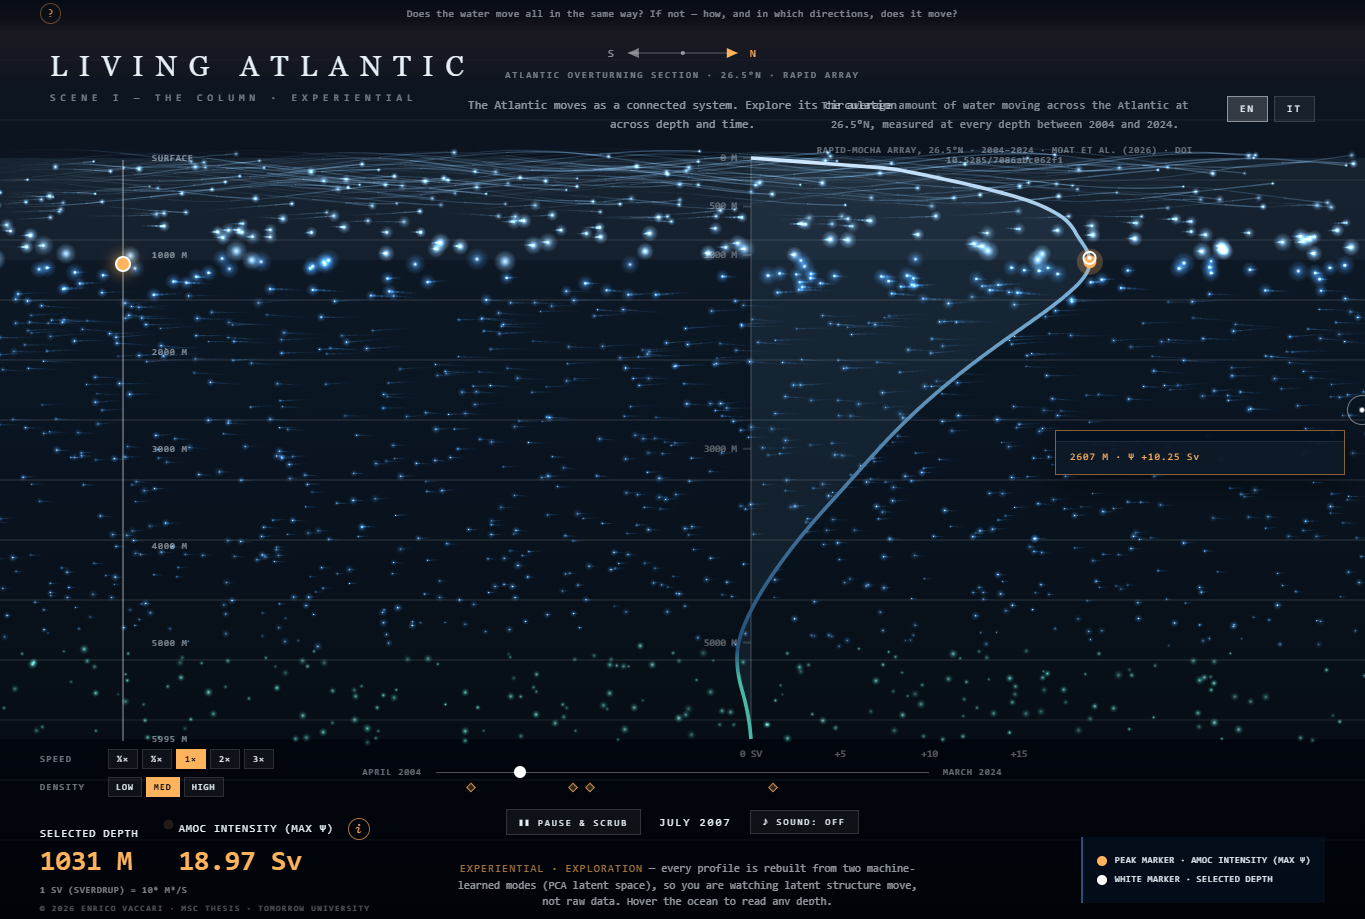
\includegraphics[width=\textwidth]{figures/viz1/viz1_thecolumn-experiential.png}
    \caption{Experiential (C2+C3): the same column set in motion.}
    \label{fig:thecolumn-experiential}
  \end{subfigure}

  \caption[The two conditions of Scene~I]{The two administered conditions of
  Scene~I, generated from the same data bundle through the same reconstruction
  function. The experiential condition introduces temporal behaviour while
  preserving the underlying structure of the static representation.}

  \label{fig:thecolumn-conditions}
\end{figure}

\paragraph{Goal.} To establish that the Atlantic at \ang{26.5}~north is not a current with a location but a quantity distributed over depth, whose parts move in opposite directions at the same moment. A viewer who leaves knowing only that the circulation is strong or weak has not received the claim.

\paragraph{Representational strategy.} The canonical profile contains the counter-flow but does not display it. To see opposing motion in the curve, a reader must know that flow direction at any depth is given by the \emph{slope} of the line rather than its height --- where the curve rises water moves north, where it falls, south --- and must read that slope by eye.

Specialists do this without noticing; non-experts, as \S\ref{sec:empirical-viz} showed, largely do not \parencite{harold2016, mcmahon2015, fischer2020}. Scene~I therefore does not help the viewer compute the derivative; it makes the derivative unnecessary, replacing the inference with motion.

\paragraph{Mapping.} The most important information here is the vertical structure (P0), so it takes spatial position across the 307 depth levels (P1).\footnote{The levels span 0--5995.1\,m and are almost uniformly spaced, at a mean interval of 19.59\,m and a maximum-to-minimum ratio of 1.03. The display corrects for no non-uniformity that is not in the data.} The counter-flow becomes a particle field advected by the local meridional velocity (P2), anomalous months become texture disturbance scored by the Isolation Forest of Chapter~\ref{ch:data_pipeline} (P3), and $\mathrm{pc}_1$ drives a synthesised pulse, off by default (P5). P4 is absent: the scene shows one trajectory and has no uncertainty to encode. Table~\ref{tab:ledger} records each element against its source in the bundle.

The particle field is driven by the derivative and never by $\Psi$ itself: driving the display from $\Psi$ would move parcels fastest exactly where the true velocity is zero, and could not depict an overturning at all. The two boundaries do not coincide and must not. $\Psi \to 0$ marks where cumulative transport vanishes, at 4346.1\,m; $v \to 0$ marks where local flow reverses, at 1050.4\,m and 5065.4\,m --- the deeper reversal sitting roughly 719\,m below the zero-crossing.\footnote{In the mean profile the peak of 16.808\,Sv sits at 1030.70\,m, with the first southward level immediately beneath it. Velocity anchors are reported at grid resolution: the derivation returns the first level where $v$ changes sign rather than an interpolated zero. The $\Psi$ zero-crossing is reported both ways: 4346.1\,m at grid resolution, 4340.85\,m interpolated.}

\paragraph{Conditions.} C1 is the canonical idiom: $\Psi$ against depth, depth downward, publication grid, peak marked, and nothing else. C2+C3 is the same column set in motion.

C1 is not a weakened comparison: it is drawn from the same bundle through the same reconstruction at the same 307 levels, and its peak marker reports 16.808\,Sv at 1030.70\,m against the 16.9\,Sv at 1030\,m published for this array \parencite{smeed2018}.

\paragraph{Fidelity.} Every profile in either condition is rebuilt through Equation~\ref{eq:reconstruction}, and the identity that makes C1 empirical is the one recorded in \S\ref{subsec:fidelity}.

\paragraph{Where the model enters.} The contribution is twofold. The static figure is an average over twenty years, and averages do not move; $\mathrm{pc}_1$ and $\mathrm{pc}_2$ make each month a point, so that walking between points reconstructs each month in turn. The motion is therefore not an animation added to a figure but the model traversing its learned trajectory, and H2 is what makes that traversal faithful rather than convenient. The model also identifies which months depart from the record, and those become perceptible as texture; everything else --- particle field, axes, peak readout --- is classical.

\paragraph{Expected contribution.} C1 shows where the Atlantic is strong on average. C2 shows what C1 contains but cannot display. C3 adds the time the model learned: the column swells toward 24.26\,Sv in January~2018 and collapses toward 5.71\,Sv in March~2013, some $3.5\sigma$ below the mean of the monthly maxima, and the peak migrates as it goes --- 1070.2\,m in the strongest month, 991.1\,m in the weakest.
\footnote{The migration is the second mode at work: $\mathrm{pc}_1$ sets how much water the column carries, $\mathrm{pc}_2$ redistributes it vertically. An earlier draft of this thesis asserted that the depth of maximum transport is stable while its magnitude varies; evaluated across the record, that is not the case.} The claim is not that the experiential condition is more attractive, but that what the static idiom fails to convey --- structure that must be inferred, change that must be imagined --- is what motion and latent time deliver directly.

\subsection{Scene II: The Engine Room}
\label{subsec:scene-engine}

\begin{quote}
\textbf{Driving Question.} \emph{Watching the ocean move from state to state over time, does it always go somewhere new, or does it sometimes pass back through where it has already been?}
\end{quote}

\begin{figure}[htbp]
  \centering

  \begin{subfigure}[t]{0.48\textwidth}
    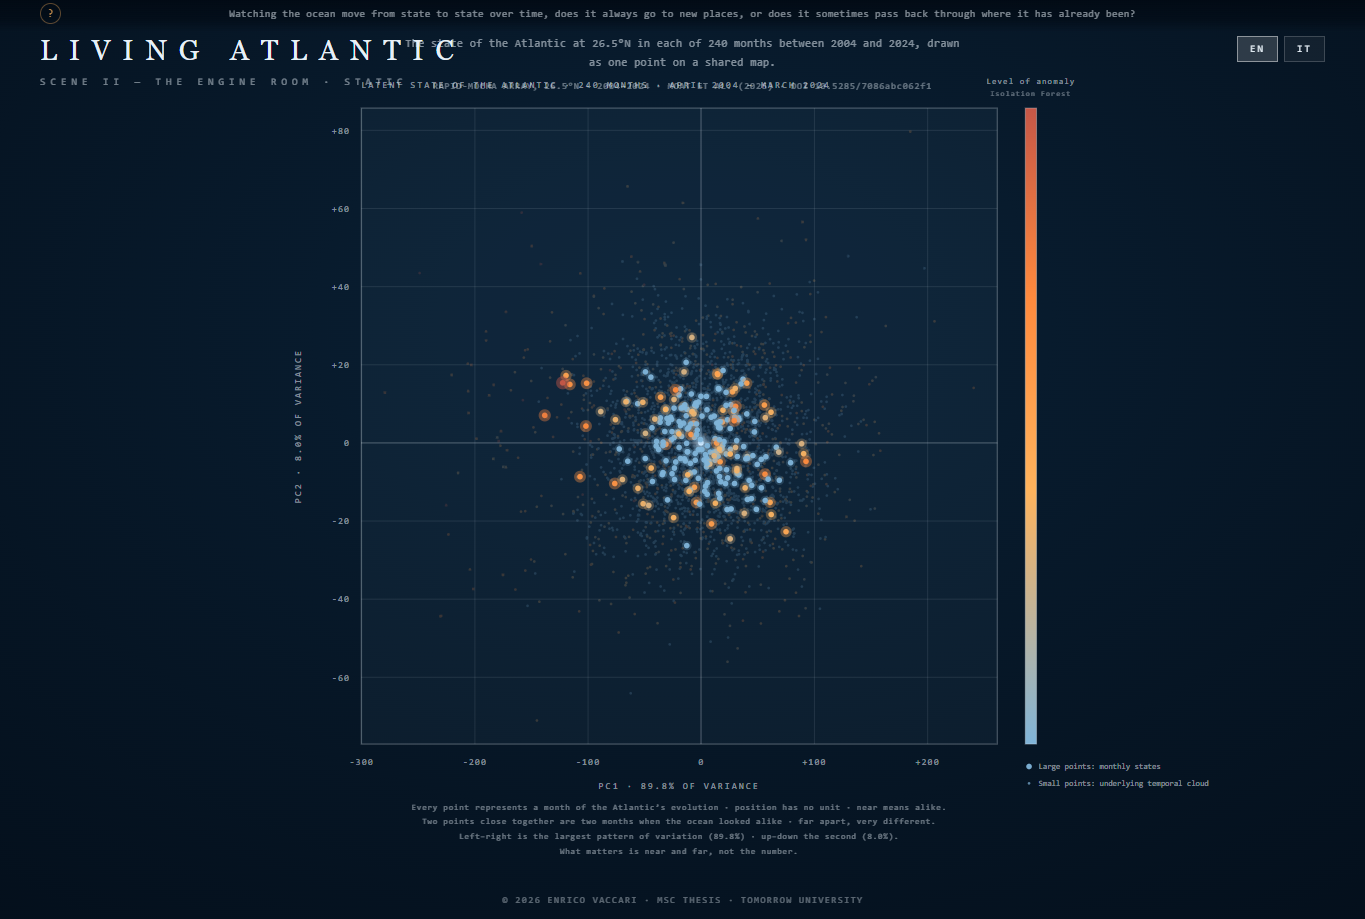
\includegraphics[width=\textwidth]{figures/viz2/viz2_theengine-static.png}
    \caption{Control (C1): the static latent-space representation.}
    \label{fig:theengine-static}
  \end{subfigure}
  \hfill
  \begin{subfigure}[t]{0.48\textwidth}
    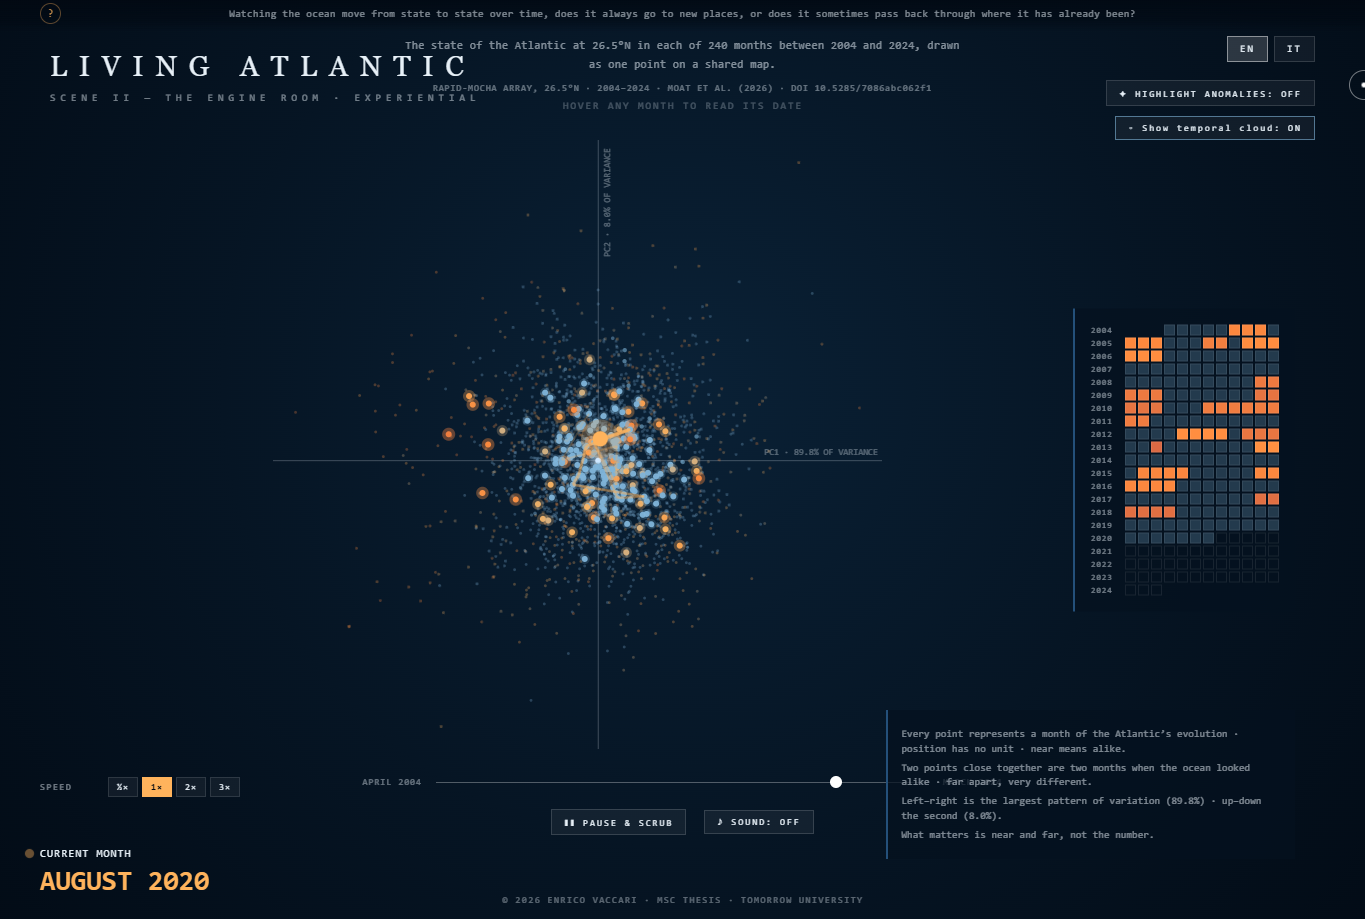
\includegraphics[width=\textwidth]{figures/viz2/viz2_theengine-experiential.png}
    \caption{Experiential (C2+C3): the evolving trajectory through latent space.}
    \label{fig:theengine-experiential}
  \end{subfigure}

  \caption[The two conditions of Scene~II]{The two administered conditions of
  Scene~II, generated from the same data bundle through the same reconstruction
  function. The static condition presents the latent structure as a fixed
  configuration, while the experiential condition reveals its temporal
  evolution.}

  \label{fig:theengine-conditions}
\end{figure}

\paragraph{Goal.} To make the latent plane of Chapter~\ref{ch:data_pipeline} an inhabitable space rather than an analyst's tool. Each month of the record is a point, and proximity means similarity. The claim the scene must deliver is that the system, left to wander, returns: it revisits states it has occupied before.\footnote{This recurrence characterises the dynamics of the present observational record, in which the AMOC oscillates within a stable regime shaped by seasonal forcing and internal variability. It is not evidence that the system cannot undergo long-term transitions.}

\paragraph{Representational strategy.} The canonical way to show a latent space is a scatter of points coloured by time \parencite{sacha2018}. That figure contains recurrence but cannot show it: two points may sit almost on top of each other while lying years apart, and a static cloud gives the eye no way to know the path left one and later arrived at the other. Recurrence is a property of the trajectory, not of the point set. Scene~II therefore walks the path in time and accumulates the visited states as a cloud.

\paragraph{Mapping.} Each month takes a position in the $\mathrm{pc}_1 \times \mathrm{pc}_2$ plane, the axes labelled with the variance each mode explains (P1). Time becomes real motion along the path, and the magnitude of month-to-month change becomes the visible violence of each step (P2): the largest steps are four times the median, and that variation is signal rather than noise to be smoothed.\footnote{The three largest steps fall on months the detect phase independently flags as anomalous --- an internal consistency recorded in Appendix~\ref{app:code}, not a claim made on screen.} Anomalous months agitate the marker (P3) and $\mathrm{pc}_1$ drives the sound (P5); P4 is again absent.

\paragraph{Conditions.} C1 is the canonical scatter: the 240 months in the plane, coloured by year through an ordered ramp, static and unannotated. C2+C3 is the same points, data and colours, set in motion. Both conditions show the same finer sub-monthly cloud behind the monthly points, so that a month reads as the average of a restless swarm rather than a single state.\footnote{From \texttt{manifold\_cloud} in the bundle. Anomaly colouring is taken from the Isolation Forest score of each point's month, not from distance to the cloud centroid; a spatial surrogate would encode ``far from centre'' as ``rare'', which is part of the reading the scene must withhold.} Neither condition draws the reconstructed profile: linking the plane back to the column would give the experimental group information the control lacks.

\paragraph{Fidelity.} The sign of each principal component is arbitrary, fixed only by the reconstruction basis, so both conditions render the plane in identical orientation: the cloud a control participant sees is the same cloud, not its mirror. Equal units on both axes keep distance on screen equal to distance in the latent space.

\paragraph{Where the model enters.} Here the model is not substrate but ground. The plane does not exist in nature: it is the basis the decomposition found, and every position in it is a learned projection. Scene~I used the latent coordinates to animate a physical object; Scene~II makes the coordinate system itself the object of attention, which is the step from expert analytics to public communication that \S\ref{sec:translate-premise} claims. The recurrence a participant looks for is a property of that learned space, perceptible only because H2 established the space is flat enough to be walked without distortion. Unlike Scene~I, nothing here would exist without the model.

\paragraph{Expected contribution.} The static scatter shows that the Atlantic occupies a bounded range of states; the experiential condition shows what it contains but cannot display --- that the system moves through that range with structure, drifting at some times and lurching at others, and that it comes back.

\subsection{Scene III: The Threshold}
\label{subsec:scene-threshold}

\begin{quote}
\textbf{Driving Question.} \emph{Do you think how much the models agree with one another has stayed the same across all the years, or has it changed?}
\end{quote}

\begin{figure}[htbp]
  \centering

  \begin{subfigure}[t]{0.48\textwidth}
    \vspace{0pt}
    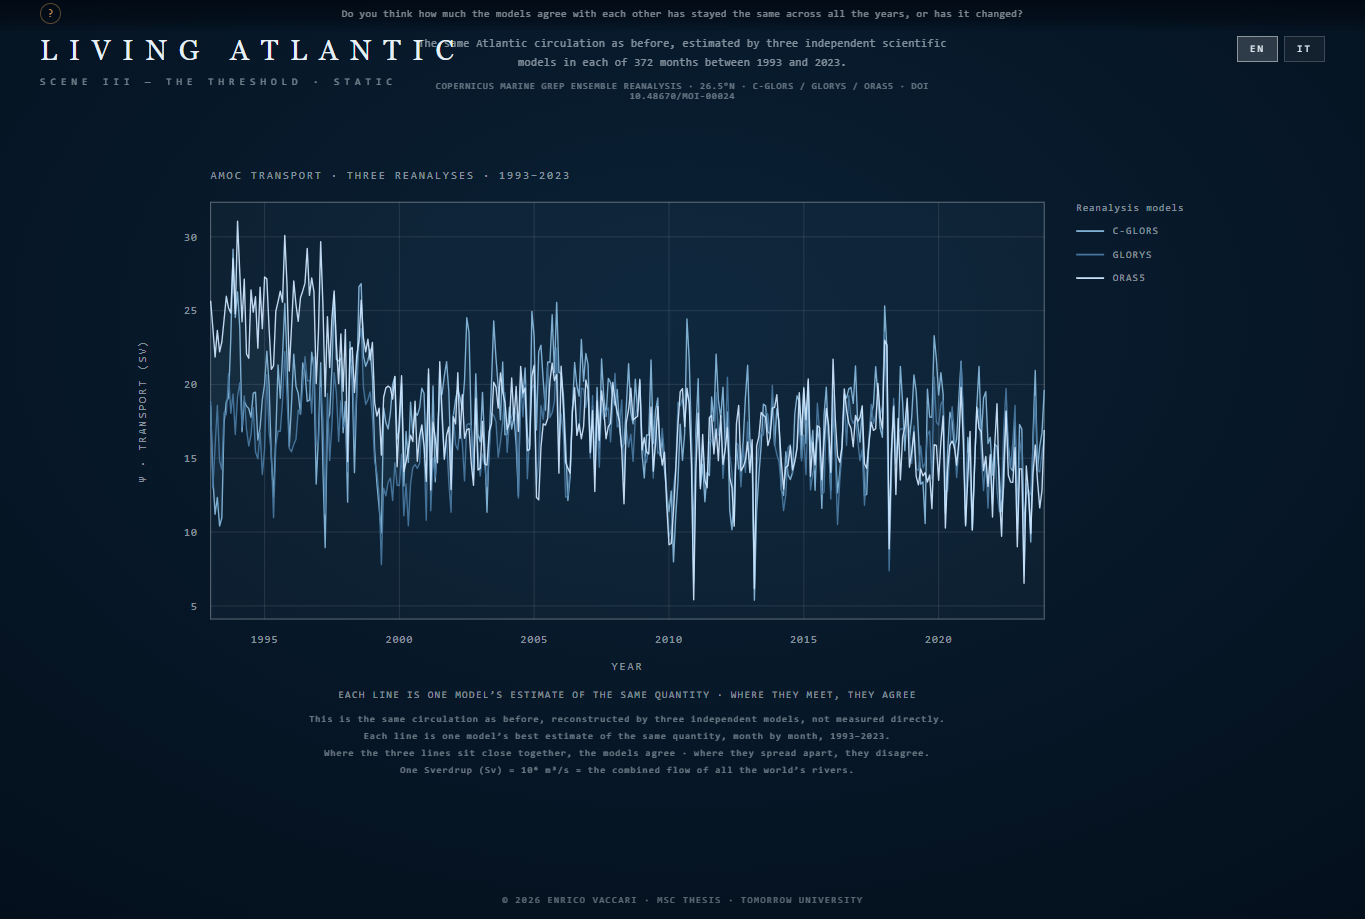
\includegraphics[width=\textwidth]{figures/viz3/viz3_thethreshold-static.png}
    \caption{Control (C1): the static representation of the threshold state.}
    \label{fig:thethreshold-static}
  \end{subfigure}
  \hfill
  \begin{subfigure}[t]{0.48\textwidth}
    \vspace{0pt}
    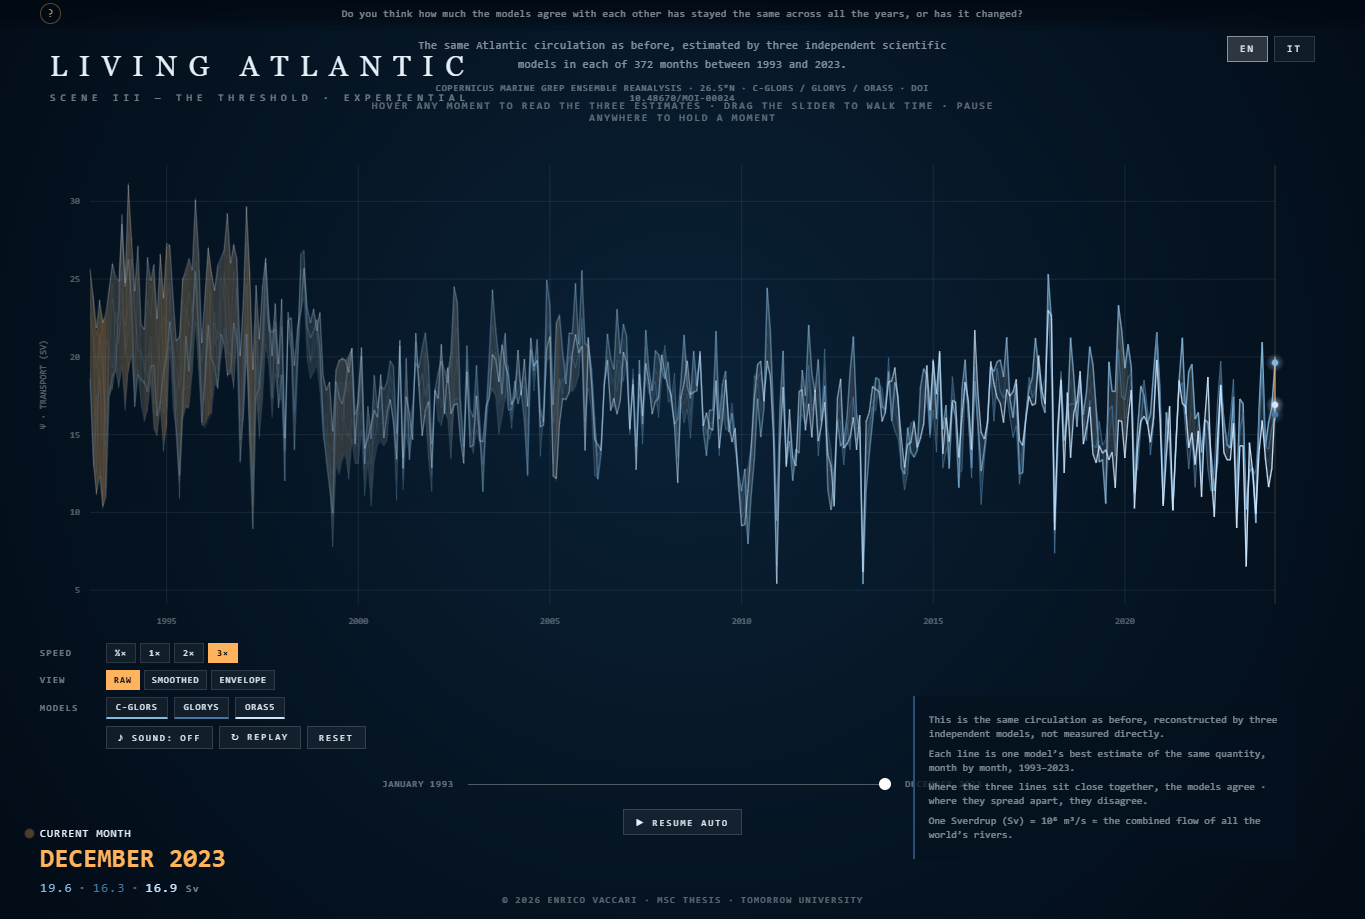
\includegraphics[width=\textwidth]{figures/viz3/viz3_thethreshold-experiential.png}
    \caption{Experiential (C2+C3): the evolving representation of uncertainty beyond the threshold.}
    \label{fig:thethreshold-experiential}
  \end{subfigure}

  \caption[The two conditions of Scene~III]{The two administered conditions of
  Scene~III, generated from the same data bundle through the same reconstruction
  function. The static condition presents the threshold structure as a fixed
  representation, while the experiential condition reveals the divergence and
  evolution of possible trajectories.}

  \label{fig:thethreshold-conditions}
\end{figure}

\paragraph{Goal.} To make uncertainty a felt quality rather than a number. Scenes~I and~II showed a quantity measured by an array in the water; Scene~III shows the same quantity reconstructed three different ways, by three ocean reanalyses that agree in the present and disagree in the past.\footnote{Copernicus Marine GREP ensemble reanalysis, members C-GLORS, GLORYS and ORAS5, monthly from January~1993 to December~2023.}

\paragraph{Representational strategy.} The canonical idiom plots the ensemble as a mean with a shaded band, or as member lines overlaid. Either contains the changing disagreement but presents it as a distance to be measured between curves --- the inferential task Scene~I sets out to remove. Scene~III instead makes disagreement a property of the medium: where the reconstructions converge the display is calm, where they diverge it becomes visibly and audibly unsettled. This realises P4, held in reserve through the first two scenes, and with it DP2.2: changing disagreement is rendered as perceptual variation rather than numerical annotation.

\paragraph{Mapping.} The most important quantity here is not the transport value but the changing disagreement, so it takes the strongest channel and becomes motion (P0). Each member's estimate holds a position against time (P1), which itself becomes real motion (P2). Uncertainty becomes animated variability (P4): turbulence, band width and colour temperature all scale with the real spread between members at each month, and none is ever printed as a figure. The same spread drives an audio texture, clean when the models agree and roughening as they part (P5). P3 is absent, anomaly not being central to the claim.

\paragraph{Conditions.} C1 draws the three member lines against time, distinguishable and named, static and unannotated: no era is shaded, no year marked. C2+C3 sets the same lines in motion and adds the living medium between them, with controls that let a viewer re-view identical data at different aggregations --- raw, smoothed over a chosen window, or the envelope alone --- and isolate any single reanalysis.\footnote{These are views of one dataset, not additional information: every aggregation is computed from the same three member series, and the raw values remain available in both conditions.}

\paragraph{Fidelity.} Every visual and auditory property is driven by the real spread between the three members at each month, and no aggregation introduces a quantity the members do not contain. The three lines are never reduced to a mean with error bars: the scene's subject is three disagreeing reconstructions, not one estimate with a margin.

\paragraph{Where the model enters.} Least of the three, and the asymmetry is instructive. The three reanalyses are physical ocean models produced by other institutions, not learned representations built for this thesis, and the spread between them is arithmetic: the machine-learning contribution of Chapter~\ref{ch:data_pipeline} does not drive this scene. What carries across is the grammar rather than the model --- the same principles that mapped latent structure to motion in Scenes~I and~II here map ensemble disagreement to animated variability, without a latent space to stand on. That the grammar survives the removal of the model is the strongest evidence available within this thesis for objective~O2.2.

\paragraph{Expected contribution.} The static plot shows that three models estimate the same quantity and do not fully agree; the experiential condition shows that the degree of agreement is itself a variable, the reconstructions parting company in the earlier record and converging as observational constraint improves, with the mean spread roughly halving between the pre-2004 decade and the years the array has been in the water.\footnote{The narrowing is gradual rather than a step at the array's installation, and the artefact marks no date; the change is left to be perceived rather than announced.} Whether a non-specialist reads that change as a change in certainty --- rather than as a decorative variation --- is what expectation~E3.2 tests.

% ============================================================
% Summary table
% ============================================================
\begin{table}[tbp]
\centering
\caption[The three scenes at a glance]{The three scenes of \emph{Living Atlantic}: the question each puts to the viewer, the principles it realises, and what the machine learning contributes. The contribution decreases across the descent --- and the grammar's survival into Scene~III, where no learned model drives the display, is the evidence for its transferability (O2.2).}
\label{tab:scene-summary}
\small
\renewcommand{\arraystretch}{1.35}

\begin{tabularx}{\textwidth}{@{}p{2.6cm} X p{2.5cm} X@{}}
\toprule
\textbf{Scene} &
\textbf{Driving question} &
\textbf{Principles} &
\textbf{What ML adds} \\
\midrule

\makecell[l]{Scene I\\The Column} &
Does the water move all in the same way; if not, in which directions? &
P0, P1, P2, P3, P5 &
The latent coordinates the profile moves along, and the anomaly scores that disturb its texture. The particle field is classical. \\

\makecell[l]{Scene II\\The Engine Room} &
Does the ocean always move somewhere new, or does it pass back through where it has been? &
P1, P2, P3, P5 &
The plane itself: the space walked is the learned basis. Nothing in the scene exists without the model. \\

\makecell[l]{Scene III\\The Threshold} &
Has the models' agreement stayed the same across the years, or changed? &
P0, P1, P2, P4, P5 &
Least of the three. The reanalyses are external physical models; the grammar carries the scene without a learned space. \\

\bottomrule
\end{tabularx}
\end{table}